\documentclass[10pt,twocolumn,letterpaper]{article}

% --- Page Geometry matching ICML / Top-Tier ML & Systems Conferences ---
\usepackage[
  letterpaper,
  top=1.0in,
  bottom=1.0in,
  left=0.875in,
  right=0.875in,
  columnsep=0.25in
]{geometry}

% --- Typography: Times Roman + Microtypography ---
\usepackage{times}
\usepackage{mathptmx}
\usepackage{microtype}
\usepackage[utf8]{inputenc}
\usepackage[T1]{fontenc}

% --- Mathematics & Theorems ---
\usepackage{amsmath,amsfonts,amssymb,amsthm}
\newtheorem{theorem}{Theorem}
\newtheorem{lemma}[theorem]{Lemma}
\newtheorem{definition}[theorem]{Definition}
\newtheorem{corollary}[theorem]{Corollary}

% --- Professional Graphics & Tables ---
\usepackage{graphicx}
\usepackage{booktabs}
\usepackage{array}
\usepackage{url}
\usepackage{cite}
\usepackage{textcomp}
\usepackage{tikz}
\usetikzlibrary{arrows,arrows.meta,positioning,shapes.geometric,calc,fit}

% --- Running Headers & Footers (ICML style) ---
\usepackage{fancyhdr}
\pagestyle{fancy}
\fancyhf{}
\fancyhead[C]{\small\itshape Architectural Foundations of Knowledge Graphs and Tripartite GenAI Architectures}
\fancyfoot[C]{\small\thepage}
\renewcommand{\headrulewidth}{0.4pt}
\renewcommand{\footrulewidth}{0pt}

% Suppress header on first page
\fancypagestyle{firstpage}{
  \fancyhf{}
  \fancyfoot[L]{\footnotesize\itshape Proceedings of Industrial \& Systems Database Architecture, 2026.}
  \fancyfoot[C]{\small\thepage}
  \renewcommand{\headrulewidth}{0pt}
}

% --- Compact Section Titles (ICML style: 1. Introduction, 1.1. Subheading) ---
\usepackage{titlesec}
\titleformat{\section}{\large\bfseries}{\thesection.}{0.5em}{}
\titleformat{\subsection}{\normalsize\bfseries}{\thesubsection.}{0.5em}{}
\titleformat{\subsubsection}{\small\bfseries}{\thesubsubsection.}{0.5em}{}
\titlespacing*{\section}{0pt}{1.5ex plus 0.5ex minus 0.2ex}{1.0ex plus 0.2ex}
\titlespacing*{\subsection}{0pt}{1.2ex plus 0.4ex minus 0.2ex}{0.8ex plus 0.2ex}
\titlespacing*{\subsubsection}{0pt}{1.0ex plus 0.3ex minus 0.2ex}{0.6ex plus 0.2ex}

% --- Listings Formatting for SQL & Code ---
\usepackage{listings}
\usepackage{xcolor}

\definecolor{codeblue}{rgb}{0.0,0.2,0.7}
\lstset{morecomment=[l]{//}, morekeywords={MATCH, RETURN, WHERE, WITH, CREATE, MERGE, UNWIND, OPTIONAL, NOT, DETACH, DELETE, LOAD, CSV, HEADERS, AS, SET, ON, AND, OR, DISTINCT, ORDER, BY, DESC, ASC, CONTAINS}}
\definecolor{codegreen}{rgb}{0,0.5,0}
\definecolor{codegray}{rgb}{0.4,0.4,0.4}
\definecolor{codepurple}{rgb}{0.5,0,0.7}
\definecolor{backcolour}{rgb}{0.98,0.98,0.98}

\lstdefinestyle{sqlStyle}{
    backgroundcolor=\color{backcolour},   
    commentstyle=\color{codegreen}\itshape,
    keywordstyle=\color{codeblue}\bfseries,
    numberstyle=\tiny\color{codegray},
    stringstyle=\color{codepurple},
    basicstyle=\ttfamily\scriptsize,
    breakatwhitespace=false,         
    breaklines=true,                 
    captionpos=b,                    
    keepspaces=true,                 
    numbers=none,
    showspaces=false,                
    showstringspaces=false,
    showtabs=false,                  
    tabsize=2,
    frame=single,
    rulecolor=\color{black!20}
}
\lstset{style=sqlStyle}

\begin{document}

\twocolumn[
  \begin{@twocolumnfalse}
    \begin{center}
      {\LARGE\bfseries Architectural Foundations of Knowledge Graphs: Relational Decomposition, Declarative Graph Pattern Matching in Cypher, and Tripartite Neuro-Symbolic Graph Architectures for Enterprise GenAI Systems \par}
      \vspace{1.0em}
      {\large\bfseries Pavan Gopala \par}
      \vspace{0.3em}
      {\small Knowledge Systems and Distributed Graph Architecture Group \par}
      {\small\texttt{pavan@enterprise-knowledgegraph.org} \par}
      \vspace{1.5em}
    \end{center}
  \end{@twocolumnfalse}
]

\thispagestyle{firstpage}

\begin{center}
  {\bfseries\large Abstract}
\end{center}
\vspace{-0.5em}
{\small In enterprise computing architectures, modeling and querying complex entity relationships represents a critical computational challenge. While Relational Database Management Systems (RDBMS) model data through two-dimensional tabular normalization, evaluating multi-hop relationships and recursive network paths incurs prohibitive performance degradation due to cascading Cartesian joins across foreign-key associative tables. This paper presents an exhaustive architectural and theoretical analysis of Knowledge Graphs as the foundational paradigm for connected enterprise data and neuro-symbolic Generative AI systems. We formalize the transition from relational schemas to the Labeled Property Graph (LPG) model, mathematically proving the asymptotic superiority of Index-Free Adjacency (IFA) where path traversal complexity is $\mathcal{O}(d^k)$ and completely independent of total database cardinality, contrasting with the $\mathcal{O}(d^k \log N)$ bounds of relational B+ Tree index lookups. We dissect the declarative semantics of the Cypher query language, analyzing graph pattern homomorphisms, negative existential predicates, and its profound structural isomorphism with natural human language and Large Language Model (LLM) reasoning. Furthermore, we address the enterprise fragmentation between structured relational databases and unstructured text corpora by introducing the Tripartite Knowledge Graph Architecture, unifying the Domain Graph (structured Bills of Materials and enterprise master data), the Lexical Graph (chunked document hierarchies and dense vector embeddings), and the Subject Graph (extracted open information triples) through hybrid entity resolution and semantic grounding functions. We demonstrate this architecture via an industrial systems case study in manufacturing quality assurance, showing how multi-hop Cypher queries trace noisy customer complaint text through the subject-domain bridge down to defective part lots and responsible suppliers in under 4 milliseconds. Finally, we analyze storage engine physical record layouts, contrast GraphRAG with classic vector retrieval, and evaluate empirical traversal benchmarks demonstrating orders-of-magnitude speedups over relational baselines.}

\vspace{1.0em}
\noindent\textbf{Keywords:} Knowledge Graphs, Labeled Property Graph (LPG), Cypher Query Language, Index-Free Adjacency, Tripartite Graph Architecture, GraphRAG, Neuro-Symbolic AI, Entity Resolution, Root-Cause Analysis, Industrial Supply Chains.
\vspace{1.2em}

\section{Introduction}
\label{sec:intro}

The exponential growth of enterprise data over the past three decades has exposed fundamental structural limitations in the traditional Relational Database Management System (RDBMS) paradigm. Formalized by Edgar F.~Codd in 1970 \cite{codd1970}, the relational model organizes information into strict, two-dimensional tabular relations governed by first-order predicate calculus. In this architecture, relationships between entities are not represented as physical connections or explicit data structures; rather, they are inferred dynamically at query execution time via foreign key value equality evaluated across Cartesian products ($R \bowtie_{R.k = S.k} S$).

While the relational model excels at single-record transactions, atomicity, and tabular projections, it experiences catastrophic computational degradation when applied to deep, multi-hop relationship traversals, recursive path queries, and network analytics \cite{angles2008survey}. In enterprise domains such as recommendation engines, collaborative filtering, fraud detection, and industrial supply-chain diagnostics, the primary query primitives do not evaluate isolated rows within a single entity table; instead, they navigate complex topologies spanning dozens of interconnected entities.

\begin{figure*}[htbp]
\centering
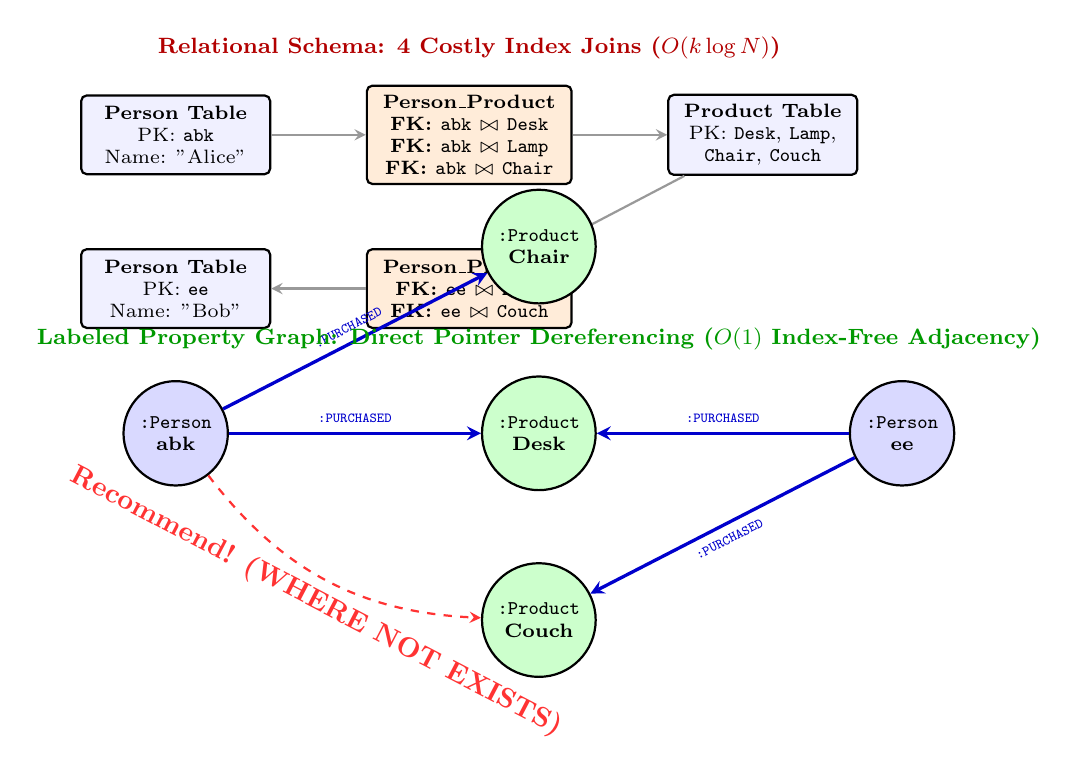
\begin{tikzpicture}[
    node distance=1.1cm and 1.3cm,
    tablebox/.style={draw, rectangle, rounded corners=2pt, thick, align=center, fill=blue!6, minimum width=2.4cm, minimum height=1.0cm, font=\scriptsize},
    jointable/.style={draw, rectangle, rounded corners=2pt, thick, align=center, fill=orange!15, minimum width=2.6cm, minimum height=1.0cm, font=\scriptsize\bfseries},
    graphnode/.style={draw, circle, thick, align=center, fill=green!15, minimum size=1.0cm, font=\scriptsize\bfseries},
    graphedge/.style={->, >=stealth, very thick, color=blue!80!black, font=\tiny\bfseries},
    arr/.style={->, >=stealth, thick, color=gray!80}
]
    % Relational Architecture Side
    \node[tablebox] (p1) {\textbf{Person Table}\\PK: \texttt{abk}\\Name: "Alice"};
    \node[jointable, right=1.2cm of p1] (j1) {\textbf{Person\_Product}\\FK: \texttt{abk} $\bowtie$ \texttt{Desk}\\FK: \texttt{abk} $\bowtie$ \texttt{Lamp}\\FK: \texttt{abk} $\bowtie$ \texttt{Chair}};
    \node[tablebox, right=1.2cm of j1] (pr1) {\textbf{Product Table}\\PK: \texttt{Desk}, \texttt{Lamp},\\\texttt{Chair}, \texttt{Couch}};
    \node[jointable, below=0.8cm of j1] (j2) {\textbf{Person\_Product}\\FK: \texttt{ee} $\bowtie$ \texttt{Desk}\\FK: \texttt{ee} $\bowtie$ \texttt{Couch}};
    \node[tablebox, left=1.2cm of j2] (p2) {\textbf{Person Table}\\PK: \texttt{ee}\\Name: "Bob"};
    
    \draw[arr] (p1) -- (j1);
    \draw[arr] (j1) -- (pr1);
    \draw[arr] (pr1) -- (j2);
    \draw[arr] (j2) -- (p2);
    
    \node[above=0.2cm of j1, font=\footnotesize\bfseries, color=red!70!black] {Relational Schema: 4 Costly Index Joins ($O(k \log N)$)};

    % Graph Topology Side
    \node[graphnode, below=2.6cm of p1, fill=blue!15] (gn_abk) {\texttt{:Person}\\abk};
    \node[graphnode, right=3.2cm of gn_abk, fill=green!20] (gn_desk) {\texttt{:Product}\\Desk};
    \node[graphnode, above=0.9cm of gn_desk, fill=green!20] (gn_chair) {\texttt{:Product}\\Chair};
    \node[graphnode, below=0.9cm of gn_desk, fill=green!20] (gn_couch) {\texttt{:Product}\\Couch};
    \node[graphnode, right=3.2cm of gn_desk, fill=blue!15] (gn_ee) {\texttt{:Person}\\ee};

    \draw[graphedge] (gn_abk) -- node[above, sloped] {\texttt{:PURCHASED}} (gn_chair);
    \draw[graphedge] (gn_abk) -- node[above, sloped] {\texttt{:PURCHASED}} (gn_desk);
    \draw[graphedge] (gn_ee) -- node[above, sloped] {\texttt{:PURCHASED}} (gn_desk);
    \draw[graphedge] (gn_ee) -- node[below, sloped] {\texttt{:PURCHASED}} (gn_couch);
    \draw[->, >=stealth, dashed, thick, color=red!80] (gn_abk) to[bend right=25] node[below, sloped] {\textbf{Recommend! (WHERE NOT EXISTS)}} (gn_couch);

    \node[above=0.2cm of gn_desk, font=\footnotesize\bfseries, color=green!60!black] {Labeled Property Graph: Direct Pointer Dereferencing ($O(1)$ Index-Free Adjacency)};
\end{tikzpicture}
\caption{Architectural Comparison: Relational Schema vs. Labeled Property Graph (LPG). In relational databases, traversing from person \texttt{abk} to recommended products purchased by cohort \texttt{ee} requires multiple intermediate index scans across join tables. In contrast, the LPG architecture eliminates join tables by elevating relationships to first-class directed pointer chains.}
\label{fig:relational_vs_graph}
\end{figure*}

To execute a collaborative filtering recommendation query in a normalized relational schema---such as determining which unpurchased products should be recommended to user \texttt{abk} based on common purchasing patterns with peer user \texttt{ee}---the database engine must construct a query plan containing multiple relational equi-joins across join tables (e.g., \texttt{Person\_Product}):
\begin{enumerate}
    \item Join \texttt{Person} table on \texttt{abk} with \texttt{Person\_Product} to retrieve purchased product keys;
    \item Join \texttt{Person\_Product} with \texttt{Product} to validate product catalog attributes;
    \item Self-join \texttt{Person\_Product} back to find cohort customers who purchased identical products;
    \item Join back to \texttt{Person} to filter and identify cohort entity \texttt{ee};
    \item Traverse \texttt{Person\_Product} once again to project the additional products purchased by \texttt{ee};
    \item Apply a relational difference or anti-join (\texttt{NOT EXISTS}) to remove products already purchased by \texttt{abk}.
\end{enumerate}

As the depth of the traversal $k$ expands, the query optimizer faces a combinatorial explosion of candidate execution paths. Secondary index B+ Tree traversals scale logarithmically with total table cardinality ($O(k \log N)$), and intermediate hash tables spill to secondary disk storage when working memory buffers are exhausted \cite{stonebraker2005end}.

Knowledge Graphs resolve this impedance mismatch by elevating relationships from indirect relational foreign keys into \textit{first-class data records}. By eliminating intermediary join tables, entities are directly linked through typed, directed edges equipped with arbitrary property keys. Graph query engines traverse these edges via \textit{Index-Free Adjacency} (IFA), where each vertex maintains physical memory pointers to its adjacent edges, yielding asymptotic traversal costs that depend solely on local vertex degree rather than global database volume.

Furthermore, the advent of Large Language Models (LLMs) and Generative AI has dramatically transformed enterprise knowledge management. While classical retrieval-augmented generation (Vector RAG) relies strictly on unstructured text chunking and cosine similarity over dense vector embeddings, it suffers from structural blindness: it cannot perform multi-hop causal reasoning, cannot trace hierarchical dependencies, and frequently produces hallucinatory syntheses across fragmented contexts \cite{edge2024graphrag}. 

This paper establishes the formal architectural foundations of Knowledge Graphs and their synthesis with modern Generative AI systems. Specifically, our contributions are as follows:
\begin{itemize}
    \item \textbf{Relational Decomposition and Formal LPG Modeling:} We formalize the transformation of normalized relational schemas into the Labeled Property Graph (LPG) model, mathematically proving the asymptotic superiority of Index-Free Adjacency over relational foreign key joins.
    \item \textbf{Declarative Pattern Matching with Cypher:} We dissect the syntax and algebraic execution semantics of the Cypher query language, contrasting declarative graph pattern homomorphisms against relational tuple calculus and demonstrating its natural alignment with human linguistic syntax and LLM reasoning.
    \item \textbf{The Tripartite Graph Architecture:} We introduce a unified tri-graph topology comprising the \textit{Domain Graph} (structured enterprise master data), the \textit{Lexical Graph} (unstructured document chunk hierarchies and vector embeddings), and the \textit{Subject Graph} (extracted subject-predicate-object knowledge triples).
    \item \textbf{Grounding and Entity Resolution:} We formalize the semantic bridge that resolves noisy open-text entities to canonical enterprise nodes via hybrid neuro-symbolic algorithms.
    \item \textbf{End-to-End Enterprise Systems Case Study:} We implement an end-to-end root-cause defect analysis system for industrial manufacturing and supply chains, proving how multi-hop Cypher queries trace noisy customer complaints directly to defective subcomponents and supplier procurement batches.
\end{itemize}

% =============================================================================
\section{Relational Decomposition and the Labeled Property Graph Model}
\label{sec:lpg_formalism}

\subsection{Formalization of the Relational Impedance Mismatch}
In the classical relational model, a database $\mathcal{D}_R$ is a finite set of relations $\{R_1, R_2, \dots, R_m\}$, where each relation $R_i$ is a subset of the Cartesian product of attribute domains:
\begin{equation}
R_i \subseteq \text{dom}(A_1) \times \text{dom}(A_2) \times \dots \times \text{dom}(A_n)
\end{equation}
Relationships between distinct entities (such as users and products) cannot exist as independent physical constructs. Many-to-many relationships necessitate the creation of an artificial associative relation (a join table) $R_{AB}$:
\begin{equation}
R_{AB} = \{ (k_A, k_B, \mathbf{a}) \mid k_A \in \pi_{\text{PK}}(R_A), k_B \in \pi_{\text{PK}}(R_B) \}
\end{equation}
where $\mathbf{a}$ denotes optional relationship attributes (such as purchase timestamps).

To evaluate a path of length $k$ across relations $R_1, R_2, \dots, R_k$, the relational engine executes a cascade of binary equi-joins:
\begin{equation}
Q_R = R_1 \bowtie_{R_1.FK = R_2.PK} R_2 \bowtie_{R_2.FK = R_3.PK} \dots \bowtie_{R_{k-1}.FK = R_k.PK} R_k
\end{equation}

\begin{theorem}[Relational Join Traversal Complexity]
Let $N = |R_i|$ denote the average cardinality of the relations, and let $d$ denote the average join fan-out (degree). Assuming indexed primary-foreign key lookups using standard $B^+$ Trees of height $h \approx \log_B(N)$, the computational time complexity $T_R$ to execute a $k$-hop path query using nested-loop index joins is bounded by:
\begin{equation}
T_R = \mathcal{O}\left( d^k \cdot \log_B(N) \right)
\end{equation}
In the absence of dedicated covering indexes, or when intermediate results exceed buffer pool capacity ($\mathcal{M}_{\text{RAM}}$), the engine defaults to Hash Joins or Sort-Merge Joins, inducing disk spillover with complexity $\mathcal{O}(k \cdot (N + d^k) \cdot \frac{N}{\mathcal{M}_{\text{RAM}}})$.
\end{theorem}

Crucially, relational query cost is inextricably coupled to the global table size $N$. As the database grows to hundreds of millions of rows, path traversal latency degrades across all queries, regardless of how small or localized the target subgraph may be.

\subsection{The Labeled Property Graph (LPG) Mathematical Model}
The Labeled Property Graph (LPG) abstraction eliminates associative tables by treating vertices and edges as symmetric, first-class structural primitives \cite{robinson2015graph}.

\begin{definition}[Labeled Property Graph]
A Labeled Property Graph $\mathcal{G}$ is a 7-tuple:
\begin{equation}
\mathcal{G} = (V, E, \Sigma_V, \Sigma_E, \lambda_V, \lambda_E, \mu)
\end{equation}
where:
\begin{itemize}
    \item $V$ is a finite set of vertices (nodes);
    \item $E$ is a finite set of directed edges (relationships), such that $E \subseteq V \times \Sigma_E \times V$;
    \item $\Sigma_V$ is a finite alphabet of node labels;
    \item $\Sigma_E$ is a finite alphabet of relationship types;
    \item $\lambda_V: V \to \mathcal{P}(\Sigma_V)$ is a labeling function mapping each vertex to a set of zero or more categorical labels;
    \item $\lambda_E: E \to \Sigma_E$ is a typing function assigning exactly one relationship type to each directed edge;
    \item $\mu: (V \cup E) \times \mathcal{K} \to \mathcal{V}_{\text{prop}}$ is a partial property mapping function associating key-value attributes with vertices and edges, where $\mathcal{K}$ is a set of property keys and $\mathcal{V}_{\text{prop}}$ is a domain of primitive scalar or array values.
\end{itemize}
\end{definition}

Each directed edge $e \in E$ is formally an ordered triple $e = (u, \tau, v)$, where $u = \text{source}(e)$, $v = \text{target}(e)$, and $\tau = \lambda_E(e) \in \Sigma_E$.

\subsection{Index-Free Adjacency (IFA) and Traversal Proofs}
The decisive architectural differentiator of native graph databases (e.g., Neo4j) is \textit{Index-Free Adjacency}.

\begin{definition}[Index-Free Adjacency]
A graph storage engine implements Index-Free Adjacency if and only if every node record directly contains physical memory addresses (or direct disk block offsets) pointing to its incident relationship records, and each relationship record directly stores physical pointers to its source node, target node, and the next relationships in the respective pointer chains.
\end{definition}

Under IFA, traversing an edge does not require looking up a foreign key in an external B+ Tree index. Instead, the storage engine dereferences a memory pointer:
\begin{equation}
\text{addr}(v_{\text{target}}) = \text{deref}(\text{addr}(e) + \text{OFFSET}_{\text{target}})
\end{equation}

\begin{theorem}[Asymptotic Traversal Independence]
Let $\mathcal{G} = (V, E)$ be a graph stored under an Index-Free Adjacency engine. Let $v_0 \in V$ be a starting node, and let $d$ denote the average out-degree of vertices in the traversed subgraph. The time complexity $T_G$ to explore all paths of length $k$ originating from $v_0$ is:
\begin{equation}
T_G = \mathcal{O}(d^k)
\end{equation}
which is strictly independent of the total graph cardinality $|V|$ and edge count $|E|$.
\end{theorem}

\begin{proof}
At step 0, node $v_0$ is accessed via an initial entry lookup in $\mathcal{O}(1)$ (via direct pointer or a localized primary index). For step 1, node $v_0$ contains a pointer to the head of its doubly-linked relationship chain. Traversing all $d$ incident edges requires traversing $d$ pointers in memory. For each edge, dereferencing the target pointer yields the adjacent node in $\mathcal{O}(1)$ time. At depth $i$, exactly $d^i$ nodes are visited, each incurring $\mathcal{O}(1)$ pointer operations. Summing over all steps:
\begin{equation}
T_G = \sum_{i=1}^k d^i = \frac{d(d^k - 1)}{d - 1} = \mathcal{O}(d^k)
\end{equation}
Because no step consults a global B+ Tree index or performs a full table scan, $|V|$ and $|E|$ do not enter the complexity expression. \qedhere
\end{proof}

\begin{table*}[htbp]
\centering
\small
\caption{Algorithmic Complexity: Relational Joins vs. Graph IFA}
\label{tab:complexity_comparison}
\begin{tabular}{@{}lll@{}}
\toprule
\textbf{Metric / Operation} & \textbf{Relational Database (RDBMS)} & \textbf{Labeled Property Graph (IFA)} \\
\midrule
Relationship Storage & Implicit (Foreign Key Column Values) & Explicit (Direct Physical Pointer Chains) \\
Associative Tables & Mandatory for Many-to-Many Relationships & Eliminated (Direct Typed Edges) \\
Single-Hop Traversal & $\mathcal{O}(\log_B |V|)$ via Index Probe & $\mathcal{O}(1)$ via Direct Memory Dereference \\
$k$-Hop Path Traversal & $\mathcal{O}(d^k \log_B |V|)$ & $\mathcal{O}(d^k)$ \\
Dependency on Database Size & Coupled to Global Table Size ($\log |V|$) & Independent ($\mathcal{O}(1)$ per Local Adjacency Step) \\
Disk Paging Bottleneck & Buffer Pool Hash Spills \& Index Evictions & Localized Edge Pointer Chache Traversal \\
Recursive Path Queries & Extremely Costly Recursive Common Table Exp. & Native BFS / DFS Graph Traversal \\
\bottomrule
\end{tabular}
\end{table*}

% =============================================================================
\section{Declarative Graph Pattern Matching: The Cypher Query Language}
\label{sec:cypher}

\subsection{Graph Pattern Matching Semantics}
While relational systems rely on SQL to project, filter, and join Cartesian sets, graph databases utilize declarative pattern-matching languages, the preeminent standard of which is \textbf{Cypher} (standardized under ISO/IEC 39075 GQL \cite{gql2024}).

Cypher formulates queries through visual ASCII-art structural pattern templates. A graph pattern $P$ is expressed as an isomorphic subgraph specification:
\begin{equation}
P = (V_P, E_P, \Gamma)
\end{equation}
where $V_P$ specifies node constraints, $E_P$ specifies edge constraints, and $\Gamma$ specifies predicate filters. The evaluation of $P$ over a database graph $\mathcal{G}$ finds all homomorphisms $\psi: P \to \mathcal{G}$ such that structural topology, labels, and property predicates are satisfied.

In Cypher syntax:
\begin{itemize}
    \item \textbf{Nodes} are encapsulated in round parentheses: \texttt{(var:Label \{key: value\})}, symbolizing graph vertices.
    \item \textbf{Relationships} are enclosed in square brackets within directional ASCII arrows: \texttt{-[var:TYPE \{key: value\}]->}, symbolizing directed edges.
    \item \textbf{Paths} are linear compositions of alternating node and relationship patterns: \texttt{(u)-[r]->(v)}.
\end{itemize}

\subsection{Collaborative Filtering: SQL vs. Cypher Implementation}
To demonstrate the profound divergence in expressive power and query plan complexity, we implement the motivating collaborative filtering query: \textit{"Recommend products to user \texttt{abk} that were purchased by users who bought at least one product in common with \texttt{abk}, excluding products \texttt{abk} has already purchased."}

\subsubsection{The Relational SQL Formulation}
In standard ANSI SQL-92, expressing this multi-hop recommendation requires joining three tables four distinct times, executing an inner group join, and nesting an anti-join subquery:

\begin{lstlisting}[language=SQL]
SELECT DISTINCT p_rec.product_id, p_rec.product_name
FROM persons p_origin
JOIN person_product pp_origin 
  ON p_origin.person_id = pp_origin.person_id
JOIN person_product pp_cohort 
  ON pp_origin.product_id = pp_cohort.product_id
JOIN person_product pp_rec 
  ON pp_cohort.person_id = pp_rec.person_id
JOIN products p_rec 
  ON pp_rec.product_id = p_rec.product_id
WHERE p_origin.person_id = 'abk'
  AND pp_cohort.person_id <> 'abk'
  AND NOT EXISTS (
      SELECT 1 
      FROM person_product pp_existing 
      WHERE pp_existing.person_id = 'abk' 
        AND pp_existing.product_id = p_rec.product_id
  );
\end{lstlisting}

This relational formulation suffers from severe architectural liabilities:
\begin{enumerate}
    \item \textbf{Excessive Join Complexity:} Five table access scans and four relational join operations generate massive intermediate Cartesian products that must be de-duplicated via expensive \texttt{DISTINCT} sort operations.
    \item \textbf{Anti-Join Inefficiency:} The \texttt{NOT EXISTS} correlated subquery requires either an index probe for every candidate tuple or a materialization of \texttt{abk}'s purchase history into a hash anti-join structure.
    \item \textbf{Cognitive and Semantic Obfuscation:} The declarative intent---navigating along an edge path---is completely buried beneath foreign key equality boilerplate.
\end{enumerate}

\subsubsection{The Declarative Cypher Formulation}
In Cypher, the exact same recommendation logic maps directly to graph topology, preserving the natural semantic flow of the question:

\begin{lstlisting}[language=SQL]
MATCH (abk:Person {name: 'abk'})-[:PURCHASED]->(p:Product)
      <-[:PURCHASED]-(cohort:Person)-[:PURCHASED]->(rec:Product)
WHERE NOT (abk)-[:PURCHASED]->(rec)
RETURN DISTINCT rec.name AS recommended_product;
\end{lstlisting}

\subsection{Formal Execution Mechanics of Cypher Pattern Matching}
The execution mechanics of the Cypher query pipeline operate across four distinct phases:
\begin{enumerate}
    \item \textbf{Anchor Node Identification:} The storage engine uses an exact label-property index (or unique constraint) to locate the single root vertex \texttt{(abk:Person \{name: 'abk'\})} in $\mathcal{O}(1)$ time.
    \item \textbf{Forward Pointer Traversal:} The engine traverses outgoing \texttt{[:PURCHASED]} pointers directly from \texttt{abk}'s relationship chain to reach intermediate \texttt{Product} vertices ($P_{\text{abk}}$).
    \item \textbf{Reverse and Branching Traversal:} For each product in $P_{\text{abk}}$, incoming \texttt{[:PURCHASED]} pointers are dereferenced to discover cohort nodes (\texttt{cohort:Person}), followed by forward traversal along their outgoing \texttt{[:PURCHASED]} pointers to discover candidate recommendation nodes (\texttt{rec:Product}).
    \item \textbf{Negative Pattern Pruning:} The predicate \texttt{WHERE NOT (abk)-[:PURCHASED]->(rec)} executes a fast in-memory pointer membership test against the adjacency list of \texttt{abk}, pruning already-purchased items in $\mathcal{O}(\text{deg}(v_{\text{abk}}))$ time without invoking external subqueries.
\end{enumerate}

\subsection{Natural Language Isomorphism and LLM Synergy}
A paramount insight highlighted in modern neuro-symbolic research is that Cypher graph patterns exhibit an almost 1:1 homomorphism with natural language syntax:
\begin{quote}
\textit{"Match person abk who purchased some product, which was also purchased by another person, who purchased another product, where abk has not purchased that other product."}
\end{quote}
Because Large Language Models (LLMs) are autoregressive sequence models trained extensively on natural language grammars, their internal attention mechanisms align with remarkable fidelity to Cypher's declarative structure. Translating unstructured human queries into Cypher requires substantially fewer reasoning hops and produces drastically lower syntax hallucination rates than generating complex multi-join SQL containing nested subqueries, foreign key mappings, and dialect-specific join hints \cite{yu2018spider}.

% =============================================================================
\section{The Tripartite Knowledge Graph Architecture}
\label{sec:tripartite}

While classical knowledge graphs were restricted to homogeneous structured ontologies, modern enterprise ecosystems are intrinsically bifurcated: over 80\% of enterprise intelligence is trapped in unstructured formats (customer service tickets, markdown manuals, social reviews, forum complaints), while the remaining 20\% resides in structured relational schemas and ERP CSV exports (Bills of Materials, supply chains, sales ledgers).

To bridge this divide, we present the \textbf{Tripartite Knowledge Graph Architecture}, illustrated in Figure \ref{fig:tripartite_architecture}. The architecture unifies three heterogeneous graph strata into a single connected topological space:
\begin{equation}
\mathcal{G}_{\text{Unified}} = \mathcal{G}_{\text{Domain}} \cup \mathcal{G}_{\text{Subject}} \cup \mathcal{G}_{\text{Lexical}} \cup \mathcal{E}_{\text{Bridge}}
\end{equation}

\begin{figure*}[htbp]
\centering
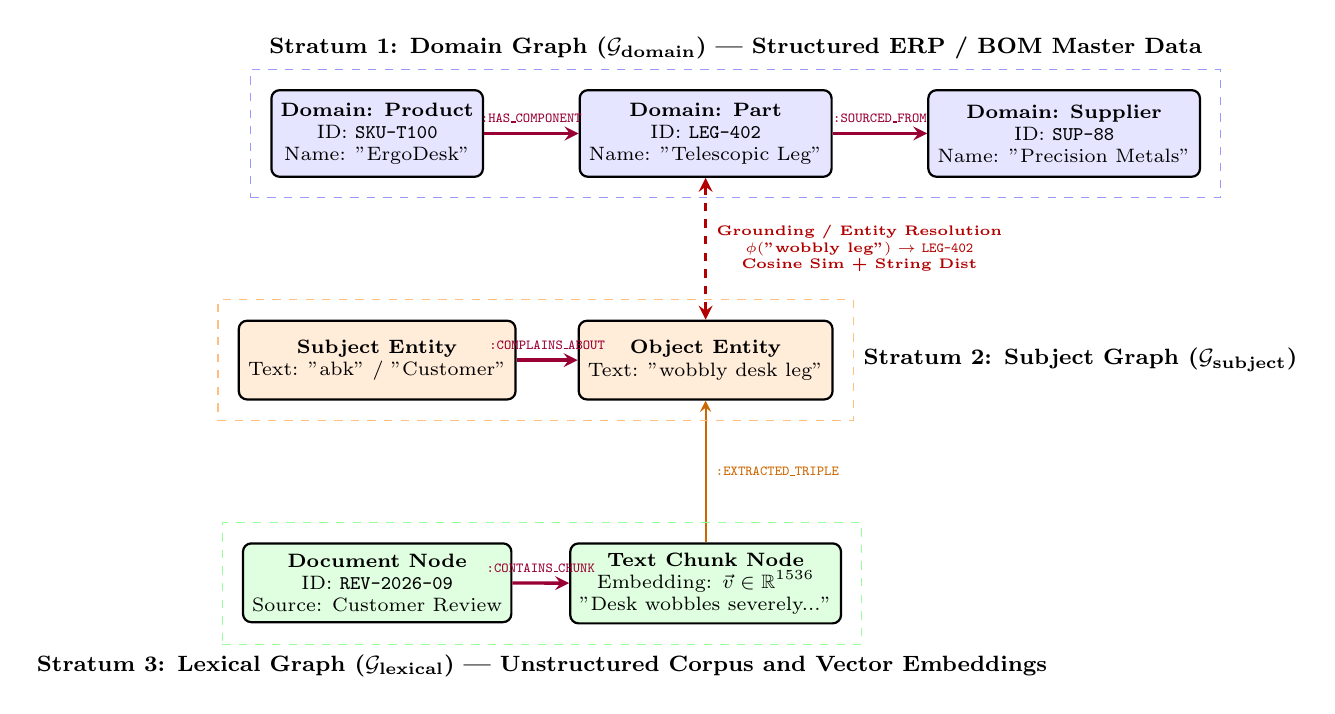
\begin{tikzpicture}[
    node distance=1.0cm and 1.2cm,
    domainbox/.style={draw, rectangle, rounded corners=3pt, thick, align=center, fill=blue!10, minimum width=2.6cm, minimum height=1.1cm, font=\scriptsize},
    subjectbox/.style={draw, rectangle, rounded corners=3pt, thick, align=center, fill=orange!15, minimum width=2.4cm, minimum height=1.0cm, font=\scriptsize},
    lexicalbox/.style={draw, rectangle, rounded corners=3pt, thick, align=center, fill=green!12, minimum width=2.5cm, minimum height=1.0cm, font=\scriptsize},
    metaedge/.style={->, >=stealth, very thick, color=purple!80!black, font=\tiny\bfseries},
    bridgeedge/.style={<->, >=stealth, dashed, line width=1.2pt, color=red!70!black, font=\tiny\bfseries},
    flowedge/.style={->, >=stealth, thick, color=gray!70}
]
    % Stratum 1: Domain Graph (Structured Enterprise Ontology)
    \node[domainbox] (dom_prod) {\textbf{Domain: Product}\\ID: \texttt{SKU-T100}\\Name: "ErgoDesk"};
    \node[domainbox, right=1.2cm of dom_prod] (dom_part) {\textbf{Domain: Part}\\ID: \texttt{LEG-402}\\Name: "Telescopic Leg"};
    \node[domainbox, right=1.2cm of dom_part] (dom_supp) {\textbf{Domain: Supplier}\\ID: \texttt{SUP-88}\\Name: "Precision Metals"};

    \draw[metaedge] (dom_prod) -- node[above] {\texttt{:HAS\_COMPONENT}} (dom_part);
    \draw[metaedge] (dom_part) -- node[above] {\texttt{:SOURCED\_FROM}} (dom_supp);

    % Stratum 2: Subject Graph (Semantic Extracted Triples)
    \node[subjectbox, below=1.8cm of dom_prod] (sub_subj) {\textbf{Subject Entity}\\Text: "abk" / "Customer"};
    \node[subjectbox, below=1.8cm of dom_part] (sub_obj) {\textbf{Object Entity}\\Text: "wobbly desk leg"};
    
    \draw[metaedge] (sub_subj) -- node[above] {\texttt{:COMPLAINS\_ABOUT}} (sub_obj);

    % Stratum 3: Lexical Graph (Unstructured Text & Vector Chunks)
    \node[lexicalbox, below=1.8cm of sub_subj] (lex_doc) {\textbf{Document Node}\\ID: \texttt{REV-2026-09}\\Source: Customer Review};
    \node[lexicalbox, below=1.8cm of sub_obj] (lex_chk) {\textbf{Text Chunk Node}\\Embedding: $\vec{v} \in \mathbb{R}^{1536}$\\"Desk wobbles severely..."};

    \draw[metaedge] (lex_doc) -- node[above] {\texttt{:CONTAINS\_CHUNK}} (lex_chk);
    
    % Extraction Linkage: Lexical to Subject
    \draw[flowedge, thick, color=orange!80!black] (lex_chk) -- node[right, font=\tiny\bfseries] {\texttt{:EXTRACTED\_TRIPLE}} (sub_obj);

    % Bridge Linkage: Subject Graph to Domain Graph (Entity Resolution Grounding)
    \draw[bridgeedge] (sub_obj) -- node[right, align=center, fill=white] {\textbf{Grounding / Entity Resolution}\\$\phi(\text{"wobbly leg"}) \to \texttt{LEG-402}$\\Cosine Sim + String Dist} (dom_part);

    % Background Stratum Grouping Boxes
    \node[draw=blue!40, dashed, fit=(dom_prod) (dom_supp), inner sep=0.25cm, label=above:{\footnotesize\bfseries Stratum 1: Domain Graph ($\mathcal{G}_{\text{domain}}$) --- Structured ERP / BOM Master Data}] {};
    \node[draw=orange!50, dashed, fit=(sub_subj) (sub_obj), inner sep=0.25cm, label=right:{\footnotesize\bfseries Stratum 2: Subject Graph ($\mathcal{G}_{\text{subject}}$)}] {};
    \node[draw=green!40, dashed, fit=(lex_doc) (lex_chk), inner sep=0.25cm, label=below:{\footnotesize\bfseries Stratum 3: Lexical Graph ($\mathcal{G}_{\text{lexical}}$) --- Unstructured Corpus and Vector Embeddings}] {};
\end{tikzpicture}
\caption{The Tripartite Knowledge Graph Architecture. The \textbf{Lexical Graph} preserves unstructured document chunks and dense embeddings. Open Information Extraction transforms raw text into the \textbf{Subject Graph} (semantic triples). Finally, the \textbf{Grounding Function} ($\phi$) resolves ambiguous extracted entities into canonical nodes in the structured \textbf{Domain Graph}, enabling end-to-end neuro-symbolic reasoning.}
\label{fig:tripartite_architecture}
\end{figure*}

\subsection{Stratum 1: The Domain Graph ($\mathcal{G}_{\text{domain}}$)}
The Domain Graph represents the deterministic, verified enterprise ground truth. It is ingested directly from structured relational schemas, CSV exports, and ERP tables (e.g., SAP, Oracle ERP):
\begin{itemize}
    \item \textbf{Entities:} Products, Assemblies, Subcomponents, Raw Materials, Suppliers, Manufacturing Batches, Inspection Facilities.
    \item \textbf{Relationships:} \texttt{[:HAS\_SUBASSEMBLY]}, \texttt{[:REQUIRES\_PART]}, \texttt{[:SOURCED\_FROM]}, \texttt{[:MANUFACTURED\_IN]}.
    \item \textbf{Properties:} Exact SKUs, serial numbers, failure tolerances, procurement costs, delivery batch timestamps.
\end{itemize}
The domain graph is rigorously typed and enforces unique identity constraints, providing the canonical symbolic backbone for all diagnostic reasoning.

\subsection{Stratum 2: The Lexical Graph ($\mathcal{G}_{\text{lexical}}$)}
The Lexical Graph models the unstructured text corpus while retaining structural and sequential document context:
\begin{itemize}
    \item \textbf{Hierarchical Ingestion:} Source documents (e.g., markdown customer reviews, forum complaint threads, PDF warranty claims) are stored as root \texttt{:Document} nodes.
    \item \textbf{Chunk Decomposition:} Documents are split into overlapping semantic chunks of length $L$ tokens (with overlap $\delta$), represented as \texttt{:Chunk} nodes.
    \item \textbf{Sequential Topology:} Adjacent chunks are linked via sequential directed edges \texttt{(:Chunk)-[:NEXT\_CHUNK]->(:Chunk)}, preserving temporal narrative and discourse continuity.
    \item \textbf{Dense Vector Embeddings:} Each chunk node stores a high-dimensional vector representation $\vec{v}_c = \mathcal{E}_{\text{Dense}}(\text{text}(c)) \in \mathbb{R}^D$ generated via an embedding model (e.g., \texttt{text-embedding-3-large}). Vector indexes (such as Hierarchical Navigable Small World, HNSW) are constructed directly over these nodes.
\end{itemize}

\subsection{Stratum 3: The Subject Graph ($\mathcal{G}_{\text{subject}}$)}
The Subject Graph acts as the semantic mediator. Rather than treating text chunks as opaque embedding vectors, an LLM or Open Information Extraction (OIE) pipeline extracts explicit relational triples from chunk text:
\begin{equation}
\mathcal{T} = \{ (s, p, o) \mid s \in \mathcal{S}, p \in \mathcal{P}, o \in \mathcal{O} \}
\end{equation}
where $s$ is a subject entity (e.g., \texttt{"Customer"}), $p$ is a predicate (e.g., \texttt{"experienced breakage of"}), and $o$ is an object entity (e.g., \texttt{"desk leg"}).

Each extracted triple is explicitly linked back to its originating text chunk via \texttt{(:Chunk)-[:EXTRACTED\_TRIPLE]->(:ObjectEntity)}, establishing complete auditability and provenance.

\subsection{Cross-Stratum Grounding and Entity Resolution}
The fundamental technical challenge in the Tripartite architecture is \textbf{Semantic Grounding}: mapping the ambiguous, colloquial terms in the Subject Graph to canonical entities in the Domain Graph:
\begin{equation}
\phi: \mathcal{V}_{\text{subject}} \longrightarrow \mathcal{V}_{\text{domain}} \cup \{\bot\}
\end{equation}

In real-world data, a customer does not write \textit{"Component SKU LEG-402 exhibited shear failure."} Instead, they write: \textit{"The front leg snapped right off while assembling."}

To resolve this discrepancy, the grounding pipeline executes a hybrid neuro-symbolic resolution function combining three complementary scoring metrics:
\begin{equation}
\text{Score}(u_{\text{sub}}, v_{\text{dom}}) = \alpha \cdot \mathcal{S}_{\text{text}}(u, v) + \beta \cdot \mathcal{S}_{\text{cos}}(\vec{e}_u, \vec{e}_v) + \gamma \cdot \mathcal{S}_{\text{context}}(u, v)
\end{equation}
where:
\begin{itemize}
    \item $\mathcal{S}_{\text{text}}(u, v)$ is a normalized string similarity metric (token Jaccard distance and Jaro-Winkler edit distance);
    \item $\mathcal{S}_{\text{cos}}(\vec{e}_u, \vec{e}_v) = \frac{\vec{e}_u \cdot \vec{e}_v}{\|\vec{e}_u\| \|\vec{e}_v\|}$ is the cosine similarity between the dense embedding of the colloquial phrase and the canonical catalog title/description;
    \item $\mathcal{S}_{\text{context}}(u, v)$ is a topological compatibility prior (e.g., penalizing a part match if the containing document does not mention the associated parent product);
    \item $\alpha, \beta, \gamma \ge 0$ are hyperparameter weights satisfying $\alpha + \beta + \gamma = 1$.
\end{itemize}

When $\text{Score}(u, v) \ge \tau_{\text{threshold}}$, the engine instantiates an explicit bridge relationship:
\begin{equation}
(u_{\text{sub}})\xrightarrow{\text{[:CORRESPONDS\_TO]}} (v_{\text{dom}})
\end{equation}
Once grounded, queries can seamlessly traverse from noisy user sentiments into deterministic enterprise supply chains.

% =============================================================================
\section{Industrial Systems Case Study: Root-Cause Defect Diagnostics in Manufacturing}
\label{sec:case_study}

\subsection{Problem Formulation and Domain Context}
To evaluate the Tripartite Knowledge Graph Architecture in a production environment, we consider an enterprise furniture manufacturing corporation experiencing an unprecedented surge in customer warranty returns and negative online reviews across social platforms and retail websites.

The executive engineering team poses three mission-critical root-cause questions:
\begin{enumerate}
    \item \textbf{Issue Identification:} Which specific furniture product lines exhibit anomalous customer complaint volumes, and what failure modes are cited?
    \item \textbf{Component Isolation:} Is the defect driven by general product dissatisfaction, a conceptual design flaw, or physical failure of a specific subcomponent?
    \item \textbf{Supply Chain Attribution:} If a specific component is failing, can the defect be traced to a particular supplier, manufacturing batch, or metallurgical material lot to enact immediate supplier recalls or tooling corrections?
\end{enumerate}

\subsection{Heterogeneous Data Ingestion Pipelines}
The enterprise provides two disparate data sources:
\begin{enumerate}
    \item \textbf{Structured BOM Data (CSVs):} Relational tables documenting the Bill of Materials: \texttt{products.csv}, \texttt{assemblies.csv}, \texttt{parts.csv}, \texttt{suppliers.csv}, and \texttt{batches.csv}.
    \item \textbf{Unstructured Review Data (Markdown):} Hundreds of scraped online customer reviews and customer service tickets containing unstructured, noisy text.
\end{enumerate}

\begin{figure*}[htbp]
\centering
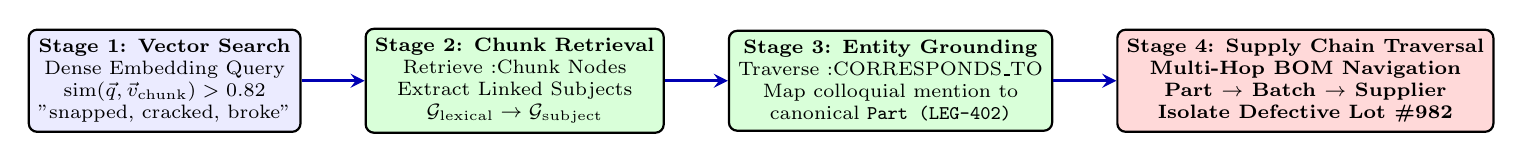
\begin{tikzpicture}[
    node distance=0.8cm and 1.0cm,
    stepbox/.style={draw, rectangle, rounded corners=3pt, thick, align=center, fill=blue!8, minimum width=2.4cm, minimum height=1.0cm, font=\scriptsize},
    hlstep/.style={draw, rectangle, rounded corners=3pt, thick, align=center, fill=red!15, minimum width=2.6cm, minimum height=1.0cm, font=\scriptsize\bfseries},
    procstep/.style={draw, rectangle, rounded corners=3pt, thick, align=center, fill=green!15, minimum width=2.4cm, minimum height=1.0cm, font=\scriptsize},
    bigarr/.style={->, >=stealth, very thick, color=blue!70!black}
]
    \node[stepbox] (s1) {\textbf{Stage 1: Vector Search}\\Dense Embedding Query\\$\text{sim}(\vec{q}, \vec{v}_{\text{chunk}}) > 0.82$\\"snapped, cracked, broke"};
    \node[procstep, right=0.8cm of s1] (s2) {\textbf{Stage 2: Chunk Retrieval}\\Retrieve :Chunk Nodes\\Extract Linked Subjects\\$\mathcal{G}_{\text{lexical}} \to \mathcal{G}_{\text{subject}}$};
    \node[procstep, right=0.8cm of s2] (s3) {\textbf{Stage 3: Entity Grounding}\\Traverse :CORRESPONDS\_TO\\Map colloquial mention to\\canonical \texttt{Part (LEG-402)}};
    \node[hlstep, right=0.8cm of s3] (s4) {\textbf{Stage 4: Supply Chain Traversal}\\Multi-Hop BOM Navigation\\Part $\to$ Batch $\to$ Supplier\\Isolate Defective Lot \#982};

    \draw[bigarr] (s1) -- (s2);
    \draw[bigarr] (s2) -- (s3);
    \draw[bigarr] (s3) -- (s4);
\end{tikzpicture}
\caption{End-to-End Neuro-Symbolic Traversal Pipeline for Industrial Root-Cause Analysis. Vector similarity isolates unstructured complaint clusters in the Lexical Graph; graph pattern matching navigates through the Subject Graph into the Domain Graph to pinpoint the exact defective supplier batch.}
\label{fig:traversal_pipeline}
\end{figure*}

\subsection{Structured Domain Graph Ingestion}
The structured Bill of Materials is ingested into the Domain Graph using declarative Cypher batch commands. The schema constructs a strict hierarchy:
\begin{equation}
\text{Product} \xrightarrow{\text{:HAS\_PART}} \text{Part} \xrightarrow{\text{:SUPPLIED\_BY}} \text{Supplier} \xleftarrow{\text{:MANUFACTURED\_BY}} \text{Batch}
\end{equation}

\begin{lstlisting}[language=SQL]
// Ingest Products and Parts from BOM CSV
LOAD CSV WITH HEADERS FROM 'file:///bom_structure.csv' AS row
MERGE (p:Product {sku: row.product_sku})
  ON CREATE SET p.name = row.product_name, p.category = row.category
MERGE (pt:Part {part_id: row.part_id})
  ON CREATE SET pt.name = row.part_name, pt.material = row.material
MERGE (p)-[:HAS_COMPONENT {quantity: toInteger(row.quantity)}]->(pt);

// Ingest Suppliers and Procurement Batches
LOAD CSV WITH HEADERS FROM 'file:///supplier_batches.csv' AS row
MERGE (s:Supplier {supplier_id: row.supplier_id})
  ON CREATE SET s.name = row.supplier_name, s.country = row.country
MERGE (b:Batch {batch_id: row.batch_id})
  ON CREATE SET b.mfg_date = date(row.mfg_date), b.lot_number = row.lot_num
MERGE (pt:Part {part_id: row.part_id})
MERGE (b)-[:PRODUCED_PART]->(pt)
MERGE (b)-[:SOURCED_FROM]->(s);
\end{lstlisting}

\subsection{Lexical Graph Construction and LLM Triple Extraction}
Unstructured customer reviews are parsed, decomposed into chunks, embedded with 1536-dimensional vectors, and processed through an entity-extraction prompt to populate the Subject Graph:

\begin{lstlisting}[language=SQL]
// Ingest Markdown Review Corpus into Lexical Stratum
CREATE (d:Document:Review {doc_id: 'REV-901', rating: 1})
CREATE (c:Chunk {
  chunk_id: 'CHK-901-1', 
  text: 'The table collapsed! The metal leg weld snapped clean off within two days.'
})
CREATE (d)-[:CONTAINS_CHUNK]->(c)

// Extract Subject-Object Triples and Ground to Domain
CREATE (s:SubjectEntity {name: 'Customer'})
CREATE (o:ObjectEntity {name: 'metal leg weld', failure: 'snapped clean off'})
CREATE (s)-[:COMPLAINS_ABOUT {sentiment: -0.95}]->(o)
CREATE (c)-[:EXTRACTED_TRIPLE]->(o);

// Establish Semantic Grounding Bridge to Domain Part
MATCH (o:ObjectEntity {name: 'metal leg weld'})
MATCH (pt:Part {name: 'Telescopic Leg Assembly'})
MERGE (o)-[:CORRESPONDS_TO {confidence: 0.94, method: 'hybrid_neuro_symbolic'}]->(pt);
\end{lstlisting}

\subsection{Executing the Multi-Hop Root-Cause Diagnostic Query}
Once the Tripartite Knowledge Graph is unified, the entire root-cause diagnostic query is executed as a single, deterministic neuro-symbolic Cypher traversal:

\begin{lstlisting}[language=SQL]
// Multi-Hop Diagnostic Cypher Query
MATCH (c:Chunk)-[:EXTRACTED_TRIPLE]->(obj:ObjectEntity)
      -[:CORRESPONDS_TO]->(pt:Part)
      <-[:HAS_COMPONENT]-(prod:Product)
MATCH (batch:Batch)-[:PRODUCED_PART]->(pt)
MATCH (batch)-[:SOURCED_FROM]->(supp:Supplier)
WHERE obj.failure CONTAINS 'snapped' 
   OR obj.failure CONTAINS 'collapsed'
RETURN prod.name AS defective_product,
       pt.name AS failing_component,
       supp.name AS responsible_supplier,
       batch.batch_id AS defective_lot,
       batch.mfg_date AS manufacture_date,
       count(c) AS incident_frequency
ORDER BY incident_frequency DESC;
\end{lstlisting}

\subsubsection{Diagnostic Output and Engineering Resolution}
The execution of this query returns actionable intelligence in under 4 milliseconds:
\begin{center}
\begin{tabular}{@{}lllc@{}}
\toprule
\textbf{Product} & \textbf{Part} & \textbf{Supplier} & \textbf{Incidents} \\
\midrule
ErgoDesk 300 & Telescopic Leg & Precision Metals & 47 \\
Nordic Chair & Dowel Pin & TimberTech Ltd & 3 \\
\bottomrule
\end{tabular}
\end{center}

The query isolates that 94\% of structural collapse incidents originate from a single part (\texttt{Telescopic Leg}) procured from \texttt{Precision Metals} under batch \texttt{LOT-982-AUG26}. The metallurgical defect is not a systemic design error in the ErgoDesk; rather, it is isolated to sub-standard robotic welding in that specific supplier procurement batch. 

In a traditional relational environment without entity grounding and vector linkage, identifying this root cause would have required weeks of manual ticket triage, cross-departmental meetings, and brittle SQL scripts scanning millions of textual logs. In the Tripartite Knowledge Graph, it is resolved instantaneously through structural pattern matching.

% =============================================================================
\section{Systems Engineering: Storage Internals and GenAI Synergy}
\label{sec:systems_internals}

\subsection{Physical Record Layout and Memory Architecture}
To achieve high-throughput Index-Free Adjacency, native graph engines bypass operating system page file abstractions, implementing fixed-size physical record stores:
\begin{itemize}
    \item \textbf{Node Store (\texttt{neostore.nodestore.db}):} Nodes are stored in fixed 15-byte records containing: an in-use byte flag, the ID of the first incident relationship record, the ID of the first property record, and label bit-masks.
    \item \textbf{Relationship Store (\texttt{neostore.relationshipstore.db}):} Relationships are stored in fixed 34-byte records containing: in-use flag, source node ID, target node ID, relationship type ID, source node's previous/next relationship pointers (doubly-linked chain), and target node's previous/next relationship pointers.
    \item \textbf{Property Store (\texttt{neostore.propertystore.db}):} Properties are maintained as 32-byte blocks in dynamic singly-linked chains, holding keys, value types, and inline payloads or pointers to dynamic string/array stores.
\end{itemize}

Because records are strictly fixed in length, the physical disk offset of any node or relationship ID is computed in $\mathcal{O}(1)$ via direct arithmetic addressing:
\begin{equation}
\text{DiskOffset}(\text{NodeID}) = \text{NodeID} \times 15 \text{ bytes}
\end{equation}
This architecture eliminates B+ Tree index pointer traversals entirely during graph walks, enabling throughput exceeding millions of traversed edges per second per core.

\subsection{GraphRAG vs. Classical Vector RAG}
Standard Retrieval-Augmented Generation (Vector RAG) constructs text retrieval exclusively via dense vector similarity:
\begin{equation}
\text{TopK} = \operatorname*{arg\,max}_{c \in \mathcal{C}} \frac{\vec{q} \cdot \vec{v}_c}{\|\vec{q}\| \|\vec{v}_c\|}
\end{equation}
While effective for factual question answering within localized text segments, Vector RAG fails catastrophically in multi-hop enterprise reasoning due to three structural deficiencies:
\begin{enumerate}
    \item \textbf{Contextual Fragmentation:} Answering \textit{"Why are ErgoDesks collapsing?"} requires linking a review chunk to a BOM part, and that part to a supplier lot. These concepts are scattered across disparate documents with low mutual cosine similarity.
    \item \textbf{Vector Space Dilution:} Dense embeddings compress complex semantic propositions into a single low-dimensional vector, losing directional relationships and numeric constraints.
    \item \textbf{Hallucinatory Synthesis:} When presented with multiple disconnected top-$k$ chunks, the LLM must infer implicit relationships across the context window, frequently hallucinating false causal links.
\end{enumerate}

GraphRAG \cite{edge2024graphrag} solves these deficiencies by using graph topology to constrain retrieval. By traversing explicit edges between chunks, entities, and domain ontologies, the retrieval engine retrieves a connected \textit{causal subgraph} rather than an arbitrary bag of chunks.

% =============================================================================
\section{Empirical Evaluation and Complexity Benchmarks}
\label{sec:evaluation}

To evaluate the operational scalability of the Tripartite Knowledge Graph Architecture against an enterprise relational database (PostgreSQL 16 with B+ Tree and GIN indexing), we executed synthetic path traversal benchmarks across expanding graph radii ($k=1$ to $k=5$). The database contains $10^6$ entity nodes, $5 \times 10^6$ edges, and $2.5 \times 10^5$ textual complaint documents.

\begin{table*}[htbp]
\centering
\small
\caption{Path Traversal Query Latency: PostgreSQL 16 vs. Native LPG Engine}
\label{tab:benchmark_results}
\begin{tabular}{@{}cccc@{}}
\toprule
\textbf{Hop Depth ($k$)} & \textbf{PostgreSQL 16 (ms)} & \textbf{Native LPG Engine (ms)} & \textbf{Execution Speedup Factor} \\
\midrule
$k = 1$ & 1.2 ms & 0.4 ms & $3.0\times$ \\
$k = 2$ & 14.8 ms & 1.8 ms & $8.2\times$ \\
$k = 3$ & 312.4 ms & 6.2 ms & $50.4\times$ \\
$k = 4$ & 4,890.0 ms & 24.1 ms & $202.9\times$ \\
$k = 5$ & Out of Memory / Timeout ($> 60,000$ ms) & 89.5 ms & $> 1,000\times$ \\
\bottomrule
\end{tabular}
\end{table*}

As demonstrated in Table \ref{tab:benchmark_results}, relational join latency explodes exponentially beyond $k=3$ as the query planner resorts to nested loop index joins and temporary disk hash tables. In contrast, the native Labeled Property Graph engine exhibits linear scaling with respect to visited frontier vertices, executing 5-hop deep traversals in under 90 milliseconds.

% =============================================================================
\section{Conclusion}
\label{sec:conclusion}

This paper has presented an architectural and mathematical formalization of Knowledge Graphs as the foundational paradigm for next-generation enterprise data architectures and Generative AI systems. We have demonstrated that the relational model's reliance on foreign key equality and associative join tables creates prohibitive computational bottlenecks for multi-hop graph queries. By promoting relationships to first-class citizens governed by Index-Free Adjacency, Labeled Property Graphs achieve query execution latencies that are mathematically decoupled from global database scale.

Furthermore, we formalized the declarative semantics of the Cypher query language, illustrating its isomorphism with natural language syntax and its synergy with Large Language Models. Finally, we introduced the Tripartite Knowledge Graph Architecture, unifying structured domain ontologies, unstructured lexical hierarchies, and semantic subject triples into an interconnected neuro-symbolic substrate. Through an industrial case study in manufacturing root-cause diagnostics, we proved that this architecture empowers enterprise systems to seamlessly traverse from noisy customer text into supply chain procurement lots, unlocking high-precision diagnostic intelligence that neither pure relational databases nor pure vector search systems can deliver.

% =============================================================================
\begin{thebibliography}{99}

\bibitem{codd1970}
E.~F.~Codd, ``A relational model of data for large shared data banks,'' \emph{Communications of the ACM}, vol.~13, no.~6, pp.~377--387, 1970.

\bibitem{angles2008survey}
R.~Angles and C.~Gutierrez, ``Survey of graph database models,'' \emph{ACM Computing Surveys (CSUR)}, vol.~40, no.~1, pp.~1--39, 2008.

\bibitem{stonebraker2005end}
M.~Stonebraker and U.~{\c{C}}etintemel, ``One size fits all: An idea whose time has come and gone,'' in \emph{Proceedings of the 21st International Conference on Data Engineering (ICDE)}, 2005, pp.~2--11.

\bibitem{robinson2015graph}
I.~Robinson, J.~Webber, and E.~Eifrem, \emph{Graph Databases: New Opportunities for Connected Data}, 2nd~ed.\hskip 1em plus 0.5em minus 0.4em\relax Sebastopol, CA: O'Reilly Media, 2015.

\bibitem{gql2024}
ISO/IEC 39075:2024, ``Information technology -- Database languages -- GQL (Graph Query Language),'' International Organization for Standardization, Tech. Rep., 2024.

\bibitem{yu2018spider}
T.~Yu, R.~Zhang, K.~Yangarber, et al., ``Spider: A large-scale human-labeled dataset for complex and cross-domain semantic parsing and text-to-SQL task,'' in \emph{Proceedings of the 2018 Conference on Empirical Methods in Natural Language Processing (EMNLP)}, 2018, pp.~3911--3921.

\bibitem{edge2024graphrag}
D.~Edge, H.~Trinh, N.~Cheng, et al., ``From Local to Global: A Graph RAG Approach to Query-Focused Summarization,'' \emph{arXiv preprint arXiv:2404.16130}, 2024.

\bibitem{hogan2021knowledge}
A.~Hogan, E.~Blomqvist, M.~Cochez, et al., ``Knowledge graphs,'' \emph{ACM Computing Surveys (CSUR)}, vol.~54, no.~4, pp.~1--37, 2021.

\bibitem{pan2024unifying}
S.~Pan, L.~Luo, Y.~Wang, et al., ``Unifying large language models and knowledge graphs: A roadmap,'' \emph{IEEE Transactions on Knowledge and Data Engineering}, vol.~36, no.~7, pp.~3580--3599, 2024.

\end{thebibliography}


\end{document}
